%results.tex

\section{Results and Discussion} \label{se:results} 
Here we present results from the first applications of local correlation to RTCC.
Results are examined
by the convergence of absorption and ECD spectra to the reference results
in Section \ref{ss:spectra}, followed by an analysis of the amplitude
dynamics in Section \ref{ss:amps}. Also explored is the effect
of localization and truncation on the orbital extent, in an
attempt to explain the deficiencies of the PNO space, in light of 
variations in the time-dependent deviations in the amplitudes from the 
ground-state.
%Section \ref{ss:alt} explores some potential solutions for building
%appropriate virtual spaces for truncation, such as considerations
%of orbital extent,
%perturbation-aware virtual spaces\cite{Crawford2019,DCunha2021}, and 
%including or focusing on the effects of the singles amplitudes. 

\subsection{Absorption and ECD Spectra} \label{ss:spectra}
\subsubsection{Absorption} \label{sss:abs}
Absorption spectra are obtained from the Fourier transform of Eq.~(\ref{eq:abs}).
Figure~\ref{fig:pno_abs} shows the normalized absorption spectrum obtained from
a reference propagation along with five PNO cutoffs. The average truncated virtual 
orbital spaces are from roughly 20\% to 90\% of the MO virtual space (see caption). 
\begin{figure} 
    \centering
    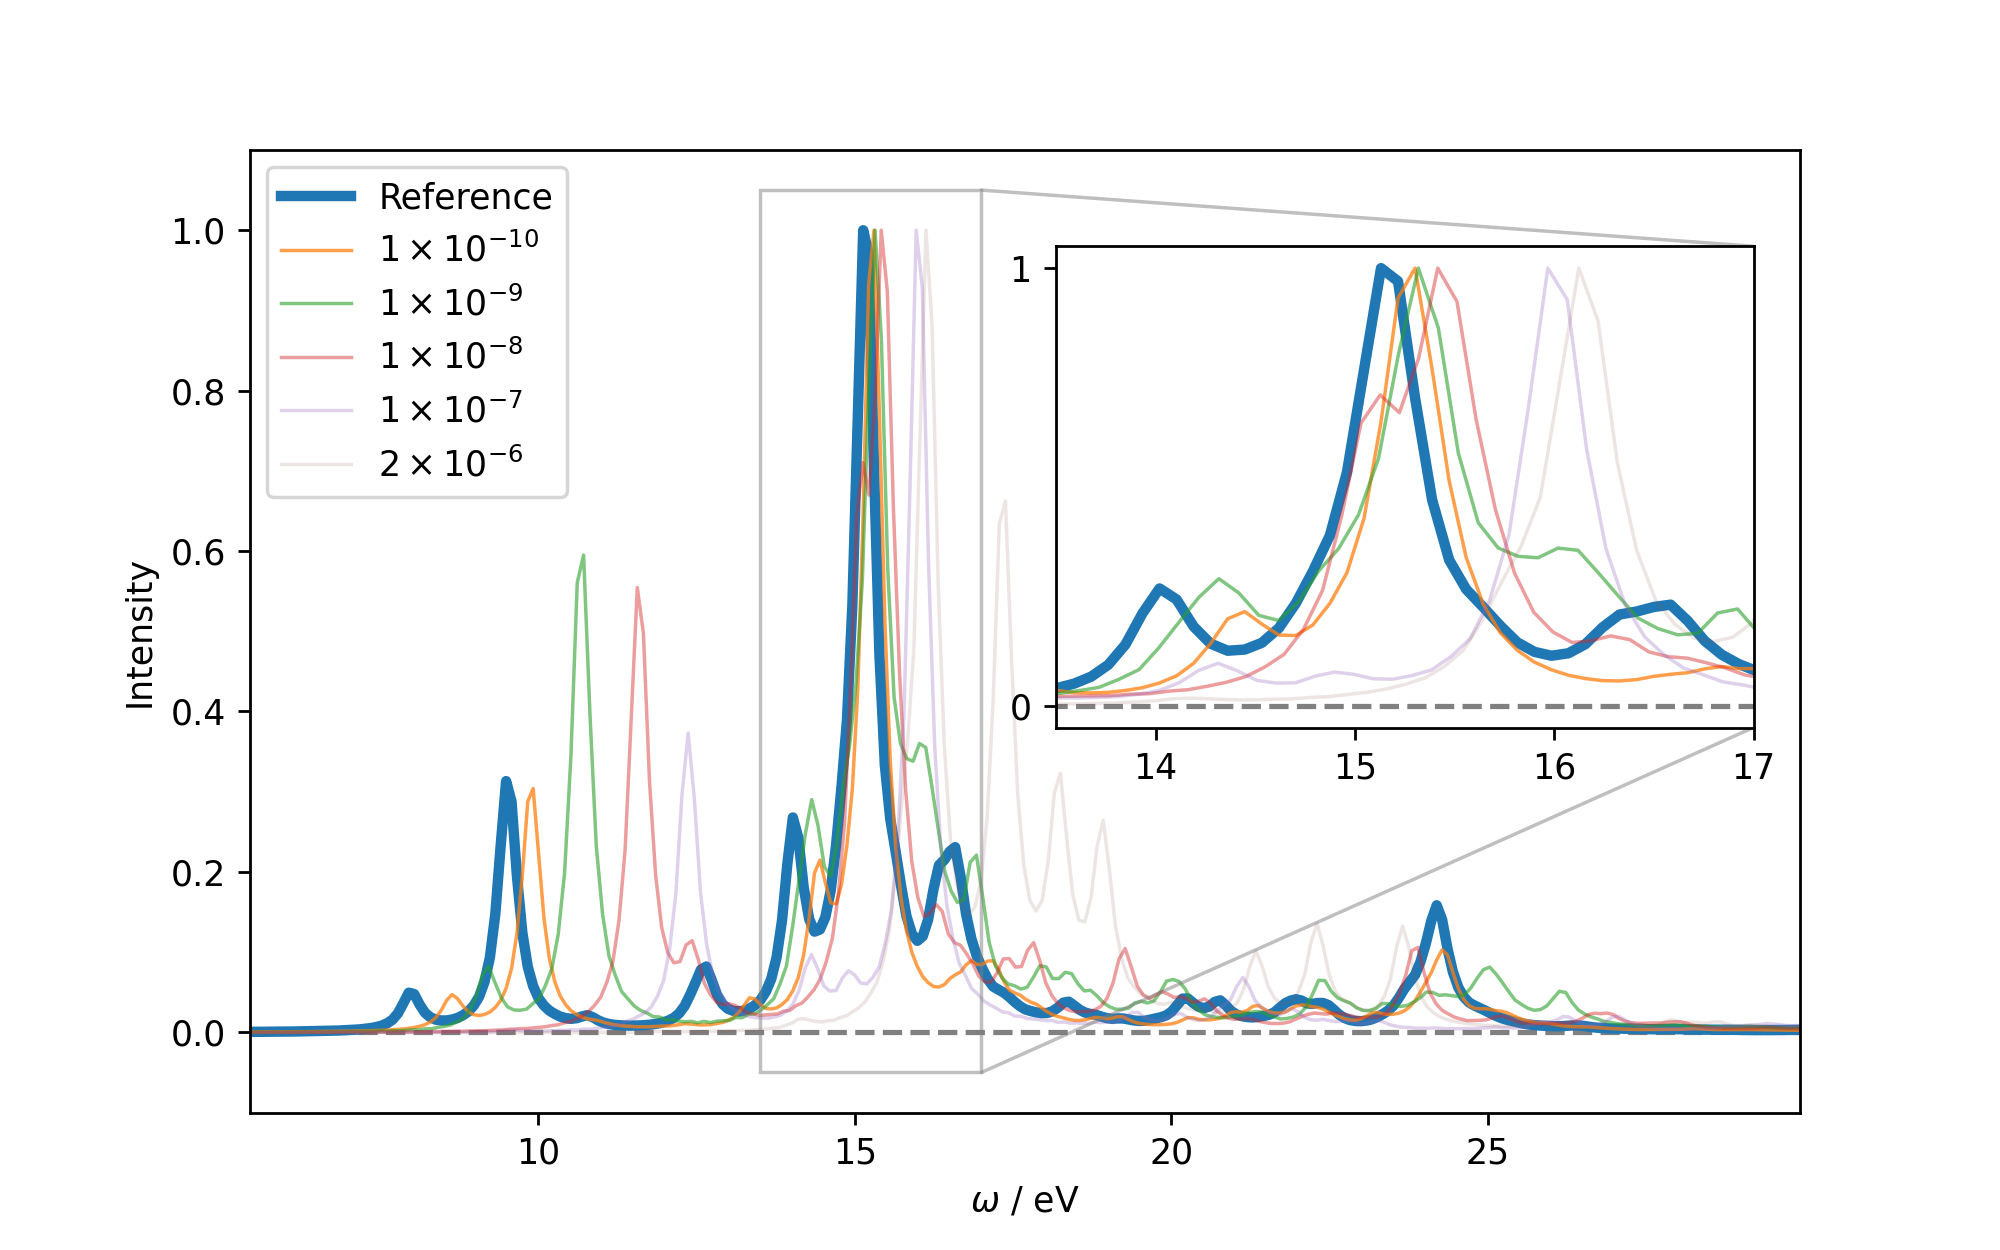
\includegraphics[scale=.6]{p3/figures/pno_abs.png}
    \caption{Reference and PNO absorption spectra of $(H_2)_4)$ for five cutoffs: 
    [$1\times 10^{-10}$, $1\times 10^{-9}$, $1\times 10^{-8}$, $1\times 10^{-7}$, 
    $2\times 10^{-6}$] corresponding to [$93\%$, $82\%$, $63\%$, $44\%$, $24\%$]
    of the MO virtual space, respectively.}
    \label{fig:pno_abs}
\end{figure}
%For all truncated PNO virtual spaces considered, the base peak appears to within 1.5 eV of the 
%reference. 
Overall, truncated PNO virtual spaces approximate the position of the base peak well,
with the smallest space predicting a base peak within 1.5 eV of the reference,
and the two largest spaces predict this peak to within 0.2 eV of the reference.
Convergence to the reference base peak occurs from the right, indicating
a lowering of excited state energies as the size of the virtual space increases. 
This trend can also be seen for the smaller peak near 10 eV. However, convergence of the shoulder 
peaks on either side of the base peak, indicated by the inset of 
Figure~\ref{fig:pno_abs}, is less predictable. Even the largest spaces considered
do not correctly predict the excitation energy, with no clear advantage to having
93\% of the virtual space as compared to just 83\% for predicting these peaks.
This trend continues into the higher-energy range of the spectrum, with the 
performance of each cutoff being nearly indistinguishable. 

Performance of the PAO space is shown in Figure~\ref{fig:pao_abs}. 
\begin{figure} 
    \centering
    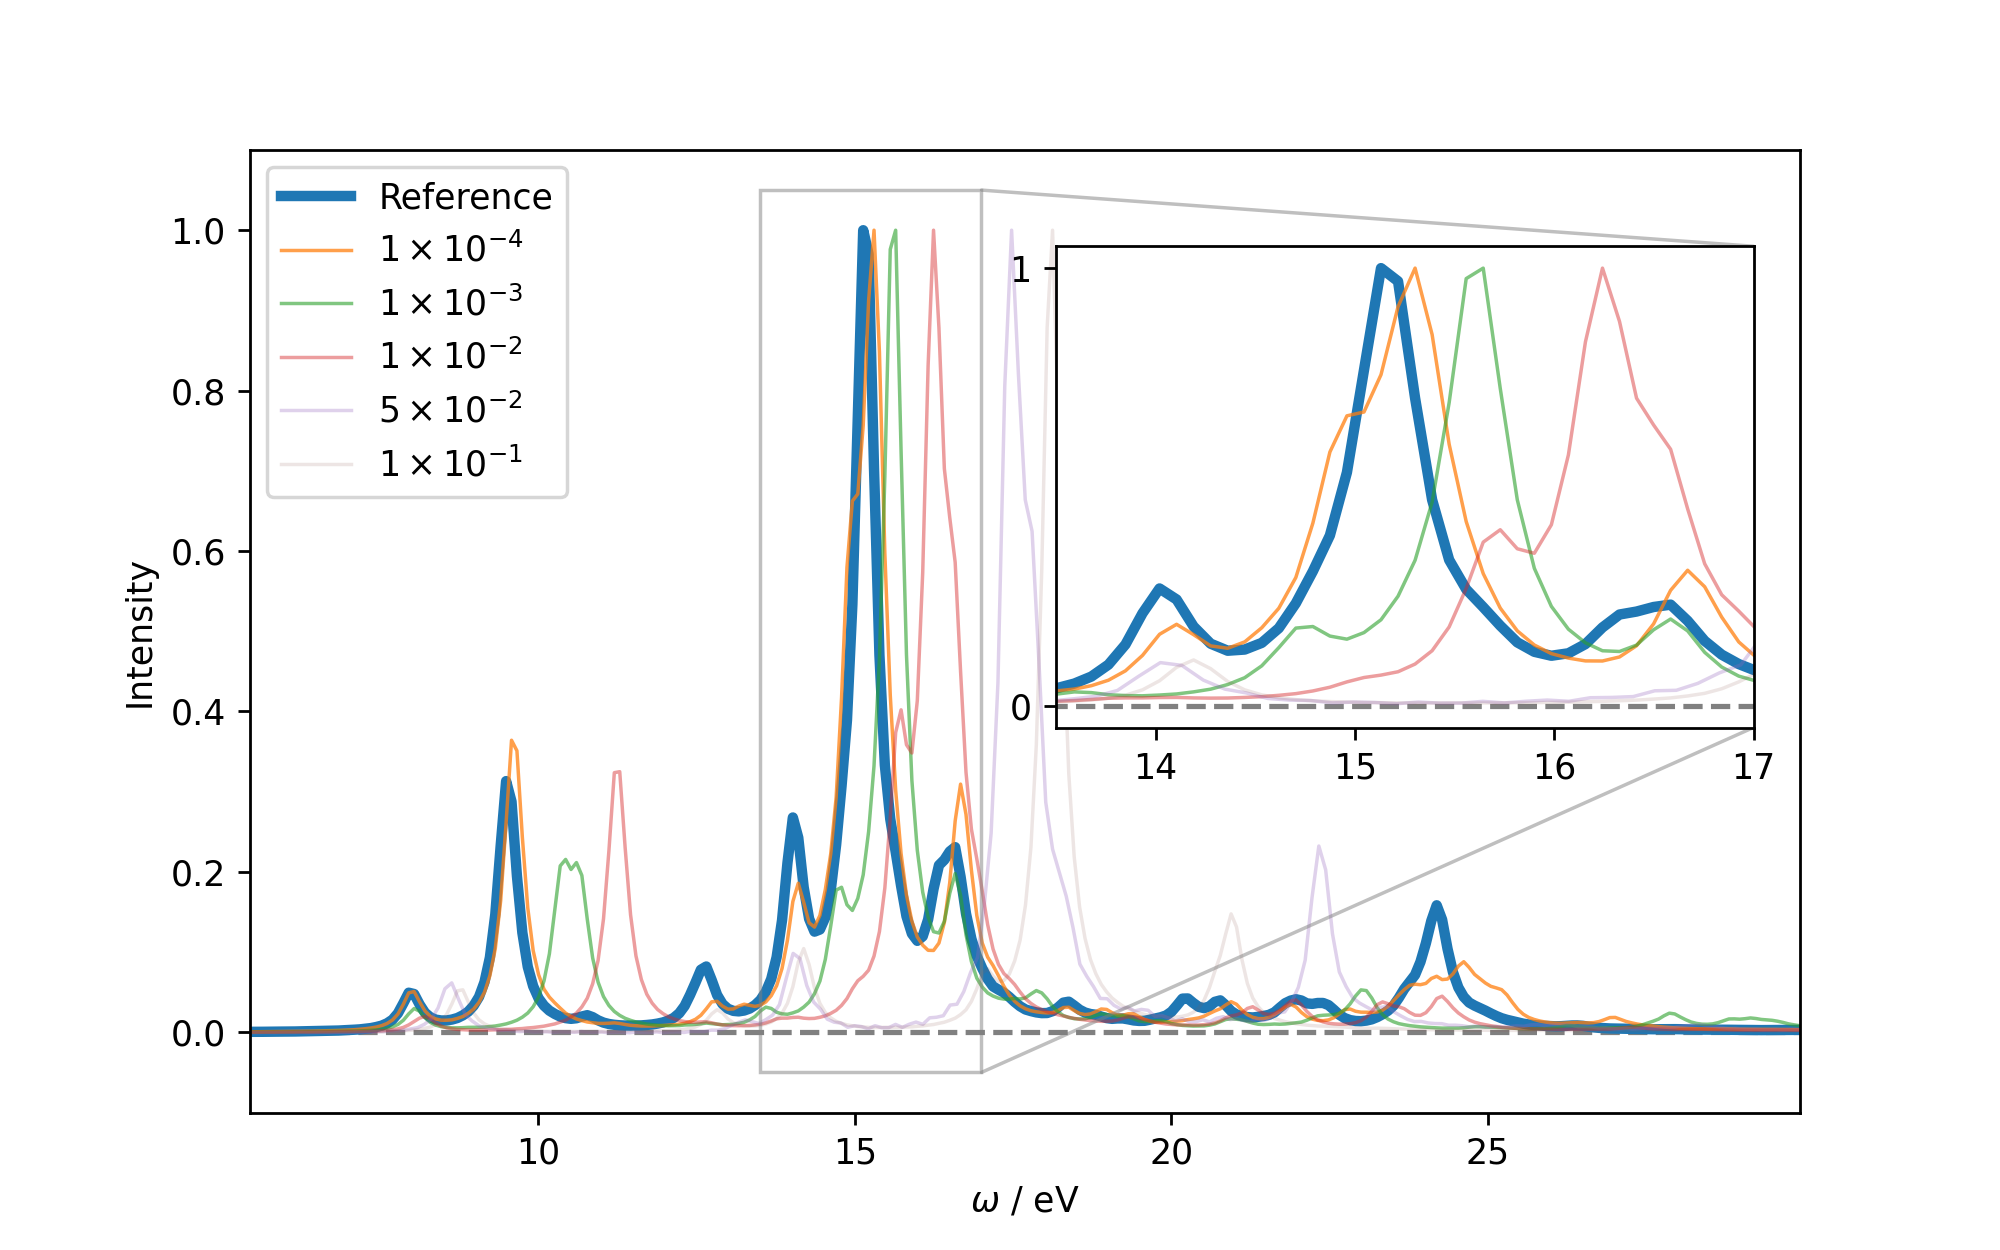
\includegraphics[scale=.6]{p3/figures/pao_abs.png}
    \caption{Reference and PAO absorption spectra of $(H_2)_4)$ for five cutoffs: 
    [$1\times 10^{-4}$, $1\times 10^{-3}$, $1\times 10^{-2}$, $5\times 10^{-2}$, 
    $1\times 10^{-1}$] corresponding to [$95\%$,$86\%$,$63\%$,$46\%$,$23\%$]
    of the MO virtual space, respectively.}
    \label{fig:pao_abs}
\end{figure}
The largest truncated PAO virtual space, on average 95\% of the MO space, accurately 
predicts the excitation energies for each major peak below 17 eV. Particularly around 10 eV, 
this is noticeably improved performance relative to the largest PNO space tested, 
with only a 2\% difference in the average size of the virtual space. 
However, accuracy rapidly declines even at 86\% of the virtual space, where the base peak
position is already worse than what was predicted with a PNO space of just 63\% of the 
MO space. Performance continues to degrade as energy increases and the average size of 
the PAO space decreases. For the final two cutoffs, at averages of 46\% and 23\% of the
MO space, the base peaks are 3 eV or more away from the reference, and no peak is 
exhibited near 25 eV. These spaces also fail to predict the second largest peak, the 
excitation just below 10 eV. 

\subsubsection{ECD} \label{sss:ecd}
Overall, neither scheme produced adequate results upon truncation of the virtual space. 
This result is not entirely surprising -- in studies of local correlation applied to 
response theory by Crawford \textit{et al}., 
\cite{McAlexander2016,Kumar2017,Crawford2019,DCunha2021} 
traditional schemes proved inaccurate for another 
electric dipole--electric dipole property, the electric polarizability.
In terms of response theory,
the polarizability (and the refractive index) is related to the \textit{real} part 
of the electric dipole--electric dipole linear response tensor 
($\boldsymbol{\alpha}_{ij}$ in Eq.~(\ref{eq:mu_exp})), 
while absorption
is related to the \textit{imaginary} part. Indeed, all linear absorptive properties
such as absorption and CD 
are related to the imaginary component of a linear response tensor, while dispersive 
properties such as refractive index and 
circular birefringence (also known as optical rotation)
are related to the real component.
\cite{Barron2004,Norman2011}
To continue, we will look at another absorptive property which is related to the mixed
electric dipole--magnetic dipole linear response tensor -- ECD.

The ECD spectrum is obtained from the Fourier transform of Eq.~(\ref{eq:ecd}).
Being a bisignate, mixed-response property, ECD is a considerable computational
challenge, similar to its dispersive counterpart circular birefringence. 
Figure~\ref{fig:pno_ecd} shows the results for an ECD spectrum in the same PNO 
orbital spaces used in the previous section.
\begin{figure} 
    \centering
    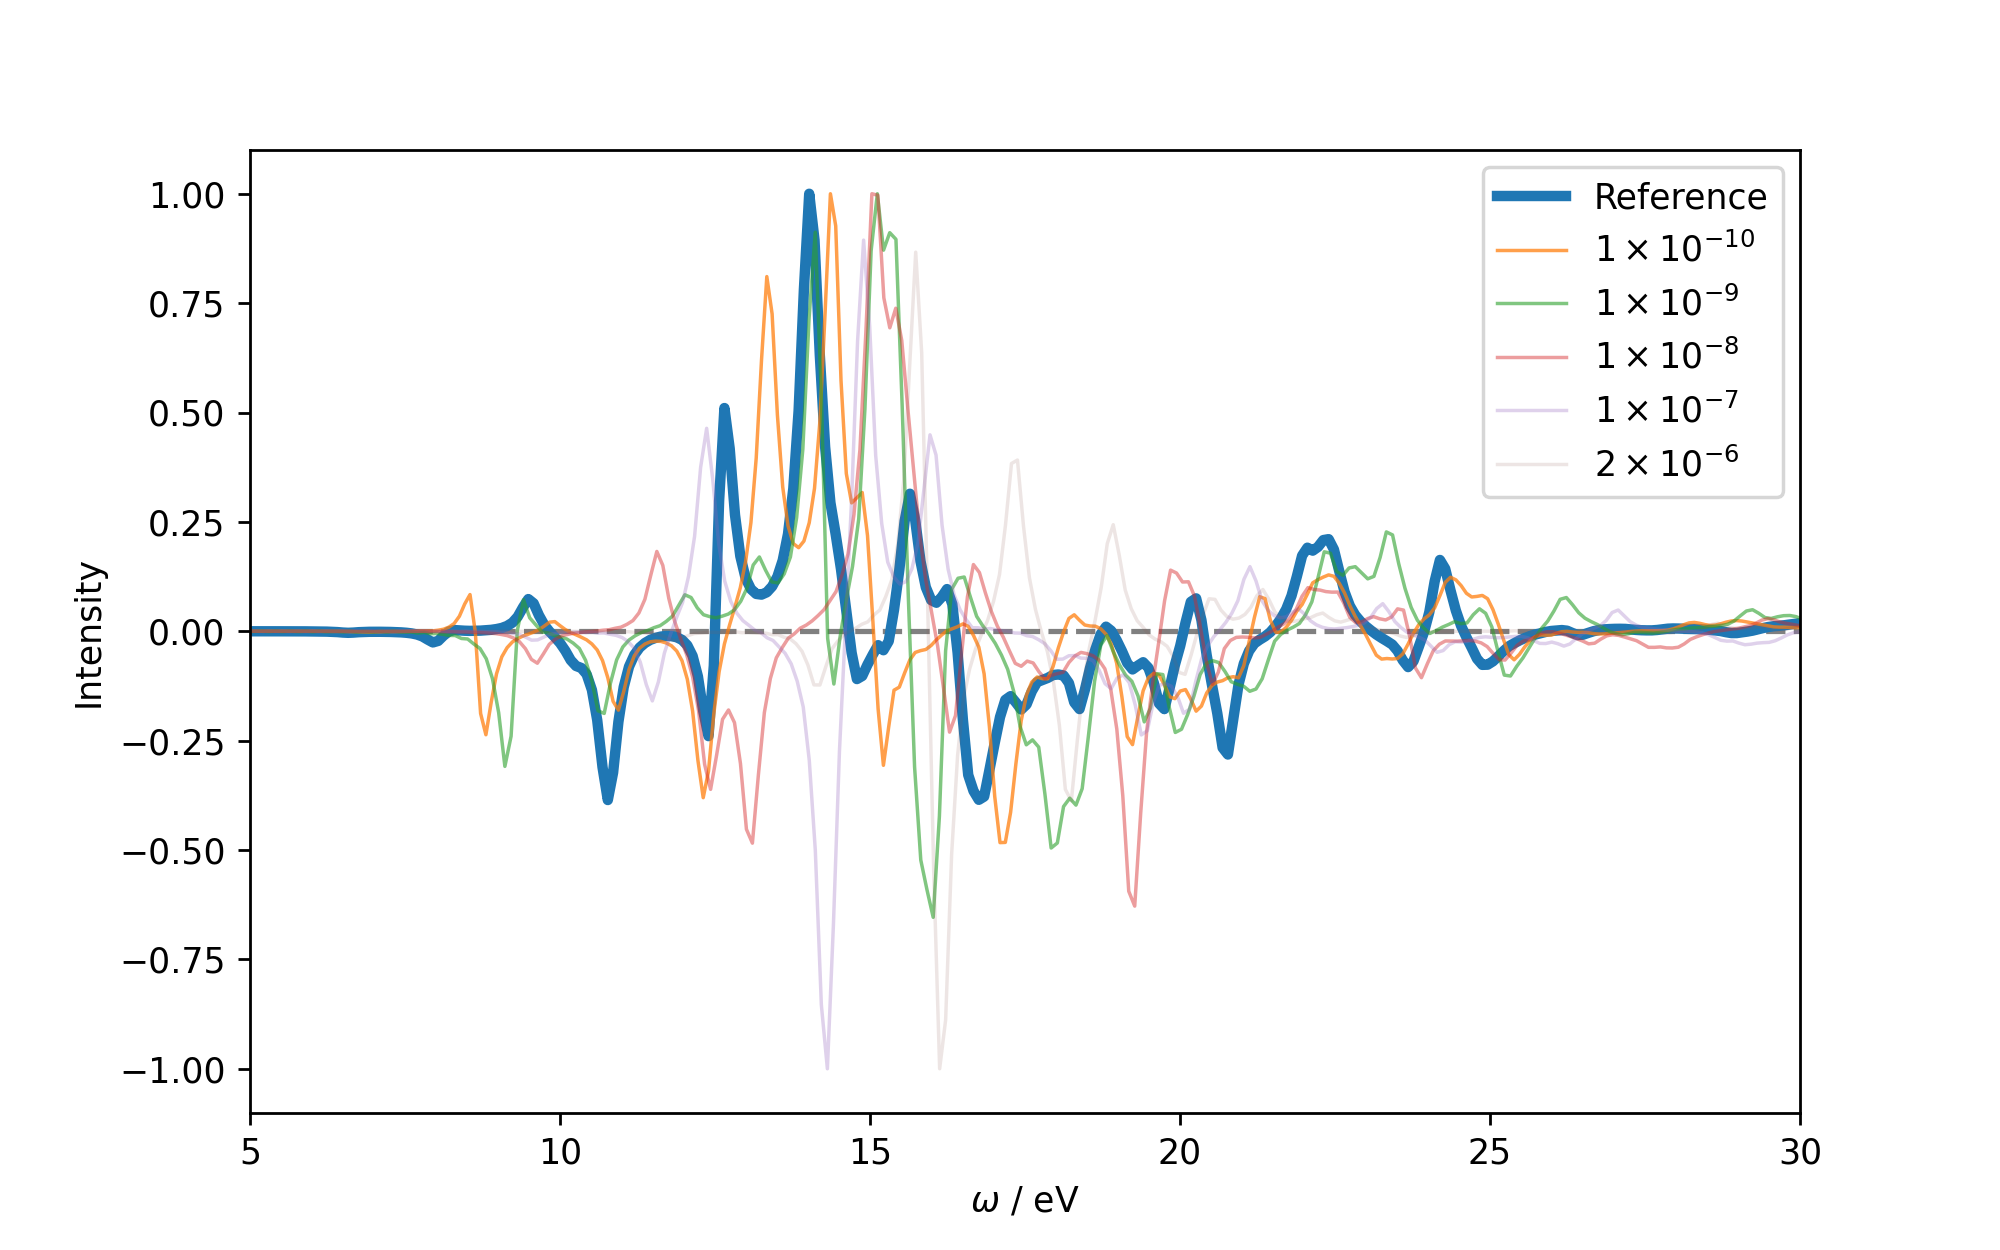
\includegraphics[scale=.6]{p3/figures/pno_ecd.png}
    \caption{Reference and PNO ECD spectra of $(H_2)_4)$ for five cutoffs: 
    [$1\times 10^{-10}$, $1\times 10^{-9}$, $1\times 10^{-8}$, $1\times 10^{-7}$, 
    $2\times 10^{-6}$] corresponding to [$93\%$, $82\%$, $63\%$, $44\%$, $24\%$]
    of the MO virtual space, respectively.}
    \label{fig:pno_ecd}
\end{figure}
The dynamic response of the magnetic dipole to the electric field in this frequency 
range is considerably more complicated than that of the electric dipole. Below 60\% of
the MO space, virtually all distinguishing characteristics of the reference 
spectrum are unidentifiable. Further, at 82\%, the base peak appears to be a pair of 
peaks, more resembling the pair of peaks appearing just above 15 eV in the 
reference spectrum, with the major peak just below 15 eV being the second strongest.
At an average of 93\%, the overall \textit{shape} of the spectrum in the 10 eV to 
20 eV range more closely resembles that of the reference; however, the excitation
energies are, in some cases, even less accurate than those of smaller PNO spaces.
The trend of lowering excited state energies with increased virtual space seen in 
Section~\ref{sss:ecd} is no longer discernible. 

As in the case of absorption, the PAO basis is not noticeably more efficient at
approximating the full MO space than the PNO space. Figure~\ref{fig:pao_ecd} 
shows the results using the same truncated PAO spaces as in Section~$\ref{sss:abs}$.
\begin{figure} 
    \centering
    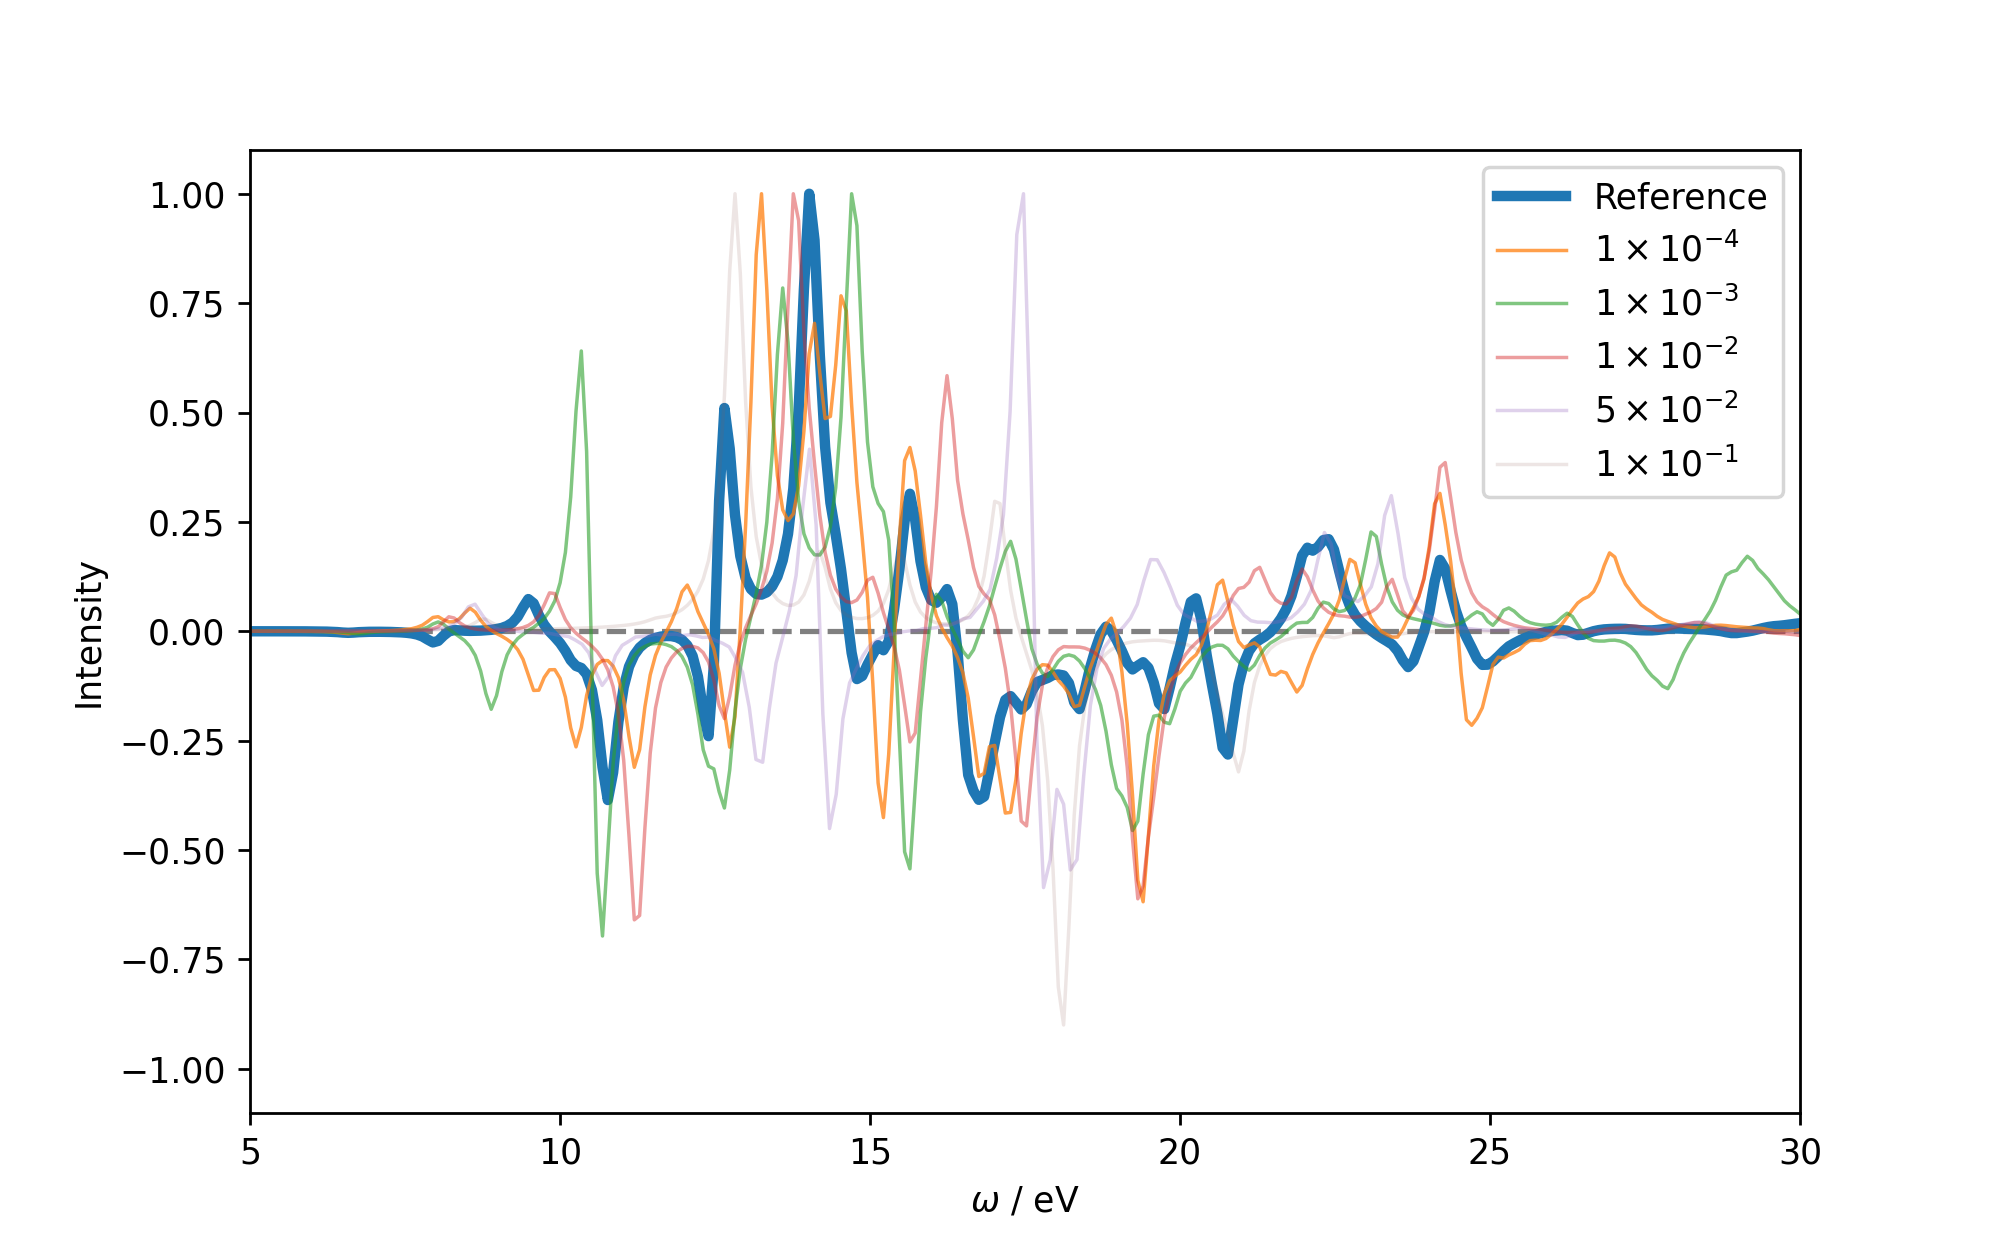
\includegraphics[scale=.6]{p3/figures/pao_ecd.png}
    \caption{Reference and PAO ECD spectra of $(H_2)_4)$ for five cutoffs: 
    [$1\times 10^{-4}$, $1\times 10^{-3}$, $1\times 10^{-2}$, $5\times 10^{-2}$, 
    $1\times 10^{-1}$] corresponding to [$95\%$,$86\%$,$63\%$,$46\%$,$23\%$]
    of the MO virtual space, respectively.}
    \label{fig:pao_ecd}
\end{figure}
The performance of the PAO basis near the base peak varies wildly with truncation,
as in the PNO case. In the low-frequency region, the PAO results are considerably 
worse -- see the two negative peaks between 10 eV and 15 eV. Curiously, the 
largest PAO spaces considered predict significant peaks above 25 eV that are not 
present in the reference, any of the PNO spaces tested, or the smaller PAO
spaces. This suggests a strong sensitivity of the response of the wave function
to the completeness threshold used for determining the occupied domains.
%fundamentally different electronic structure in the
%presence of the perturbing field, which is a direct result of the charge-based 
%completeness threshold used for determining the occupied domains.
%albeit at very large frequencies which are of little practical use.

\subsection{Amplitude Dynamics} \label{ss:amps}
As evidenced by the preceding data, the truncated PNO and PAO virtual spaces do not
efficiently model the wave function in the presence of a perturbing EMF. As noted in
Section~\ref{sss:abs}, these shortcomings are well-documented in the case of response
theory. However, a real-time formalism offers the opportunity to analyze the wave 
function in great detail over time, perhaps shedding light on \textit{where} and 
\textit{how} the locally correlated wave functions are deficient. The following
section will scrutinize the $t_\mu$ and $\lambda_\mu$ amplitudes of 
Eqs.~(\ref{eq:t_mu}) and (\ref{eq:l_mu}), respectively, in hopes of determining the 
important fluctuations in the wave function and whether these spaces sufficiently 
capture these changes.

Response to external perturbations by the CC amplitudes give rise to
dynamic energetics and properties. In the past, distributions of perturbed amplitudes
(relative to their ground-state counterparts) have been used to justify the 
difficulty in computing response functions with local correlation methods in the 
frequency domain. 
\cite{McAlexander2016,Crawford2019,DCunha2021} 
However, initial findings show that in RTCC, the relative distribution of amplitudes 
by magnitude is not significantly impacted.\cite{Crawford2019} 
Despite this, typical means of exploiting amplitude
sparsity have been shown to be inefficient by the preceding sections. 
First, to understand the response of 
the amplitudes to the external perturbation, we plot the 
change in the norm of the amplitude tensors relative to the ground-state amplitudes 
as a function of time in Figure~\ref{fig:norm}.
\begin{figure} 
    \centering
    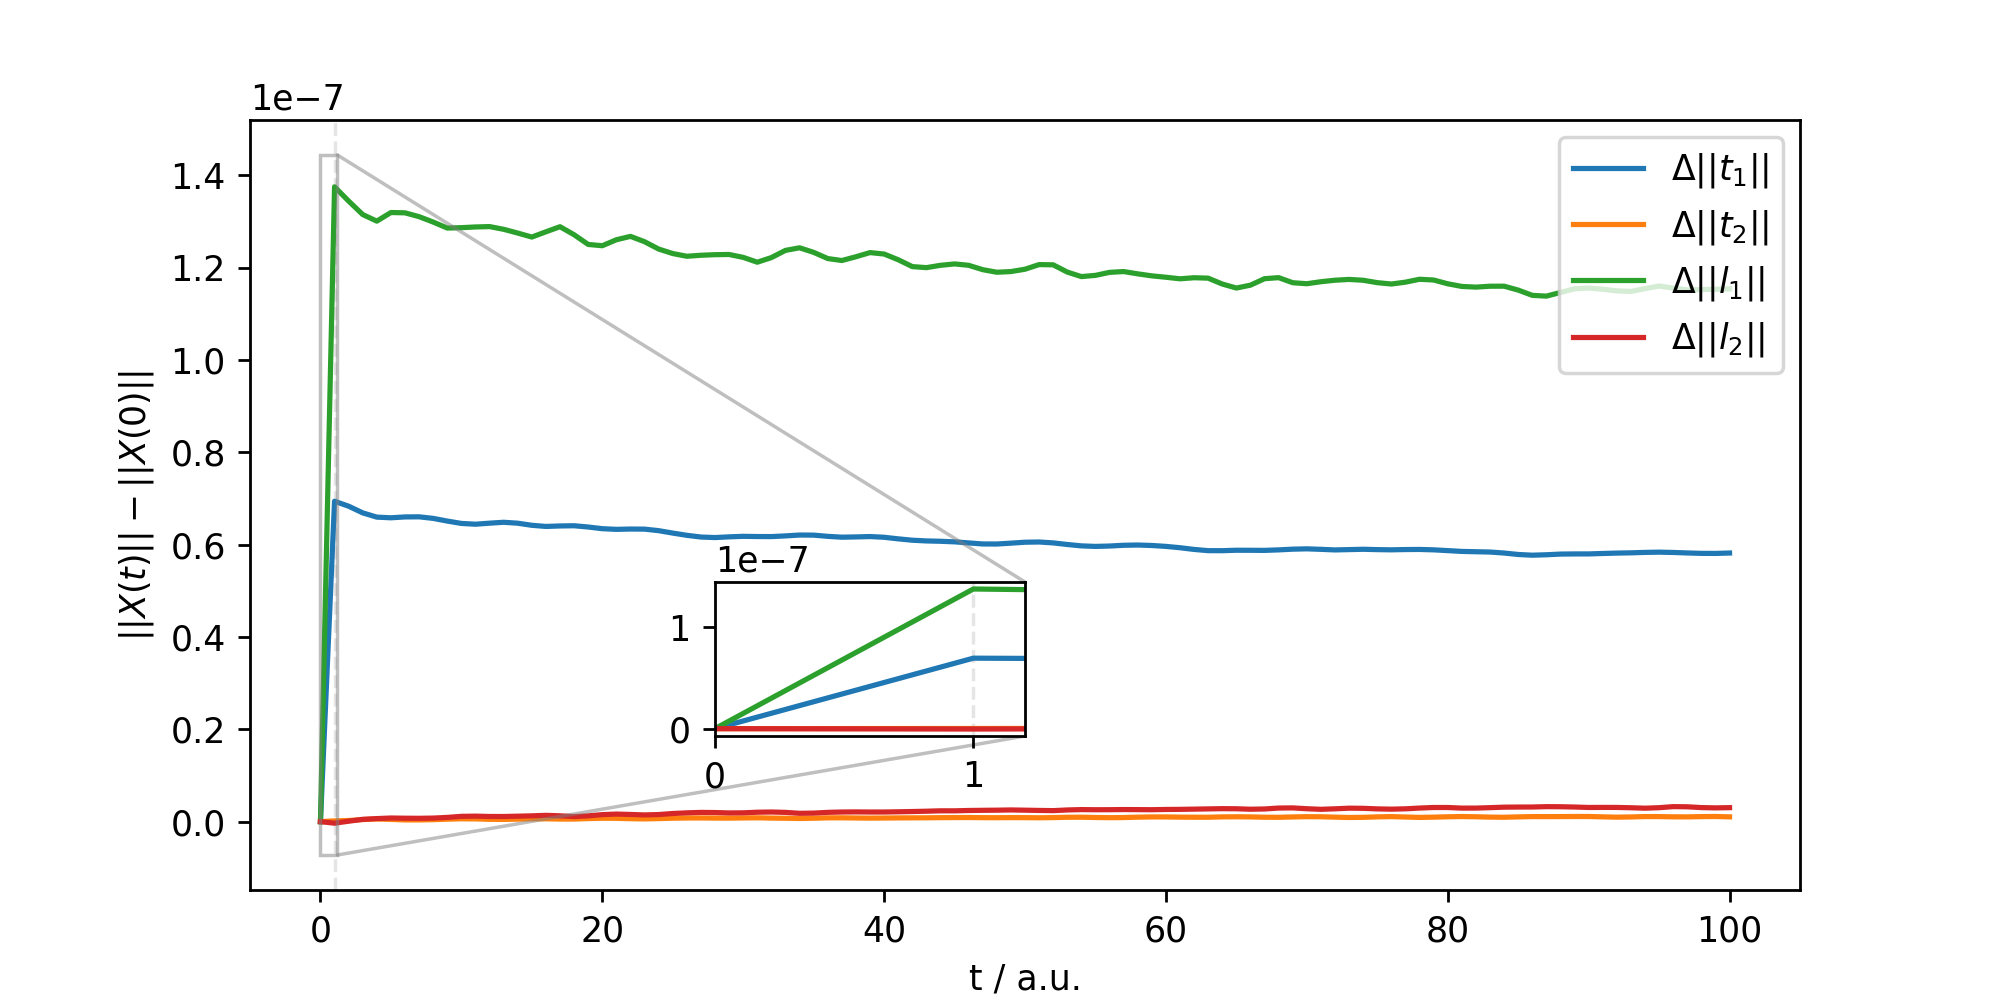
\includegraphics[scale=.6]{p3/figures/amp_norm.png}
    \caption{Time-dependent change in the norm of the amplitude 
    tensors relative to the ground-state amplitudes.
    (Field and step parameters remain unchanged, and 
    the amplitude norm is taken at every 1 a.u.)}
    \label{fig:norm}
\end{figure}
Results for the untruncated PNO and PAO spaces are identical to those
for the MO space, as the unitary transformations resulting from untruncated localized virtual spaces
in Eqs.~(\ref{eq:rotate}) preserves the tensor norm.
Amplitude norms from propagations carried out in truncated PNO and PAO spaces
are nearly indistinguishable (see SI).

Figure~\ref{fig:norm} shows that the magnitude of the response by the wave function
is predominantly within the singles amplitudes $t_1$ and $\lambda_1$. This is 
consistent with the notion that singles are paramount for the computation of 
response properties.\cite{Christiansen1995,Koch1997} However, the form of Eq.~(\ref{eq:pair_D})
does not include any contributions by singles, due to being built from MP2-level
amplitudes where singles do not contribute until at least the second order 
in the wave function and fourth order in the energy. This suggests that even in schemes
which seek to include the EMF perturbation in the construction of the reduced virtual space,
such as PNO++,\cite{DCunha2021} response of the singles should be considered.

Aside from the matrix norm, we can also inspect the individual amplitudes to track
their evolution in time. The heat maps in Figure~\ref{fig:amps} show the difference 
in $t_1$ amplitudes, relative to the ground state, for three time steps selected 
from the first 100 a.u. of the simulation.
\begin{figure}
    \begin{subfigure}{.5\textwidth}
        \centering
        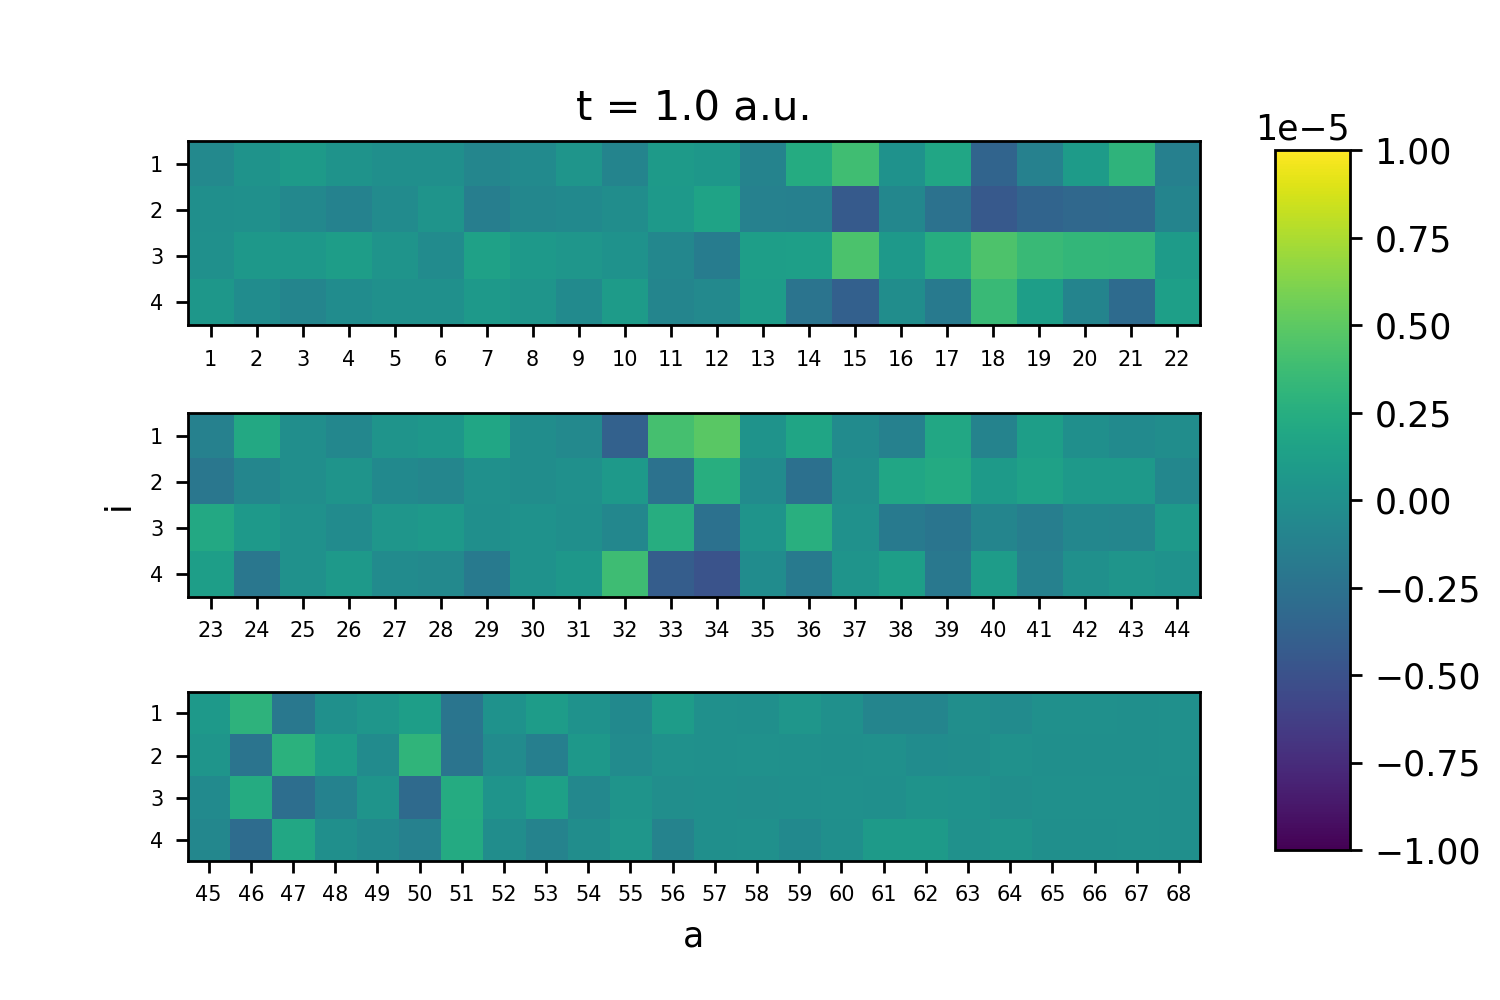
\includegraphics[scale=0.5]{p3/figures/MO_delta_t1_1.png}
        \caption{}
        \label{fig:MO_t1_1}
    \end{subfigure}%
    \begin{subfigure}{.5\textwidth}
        \centering
        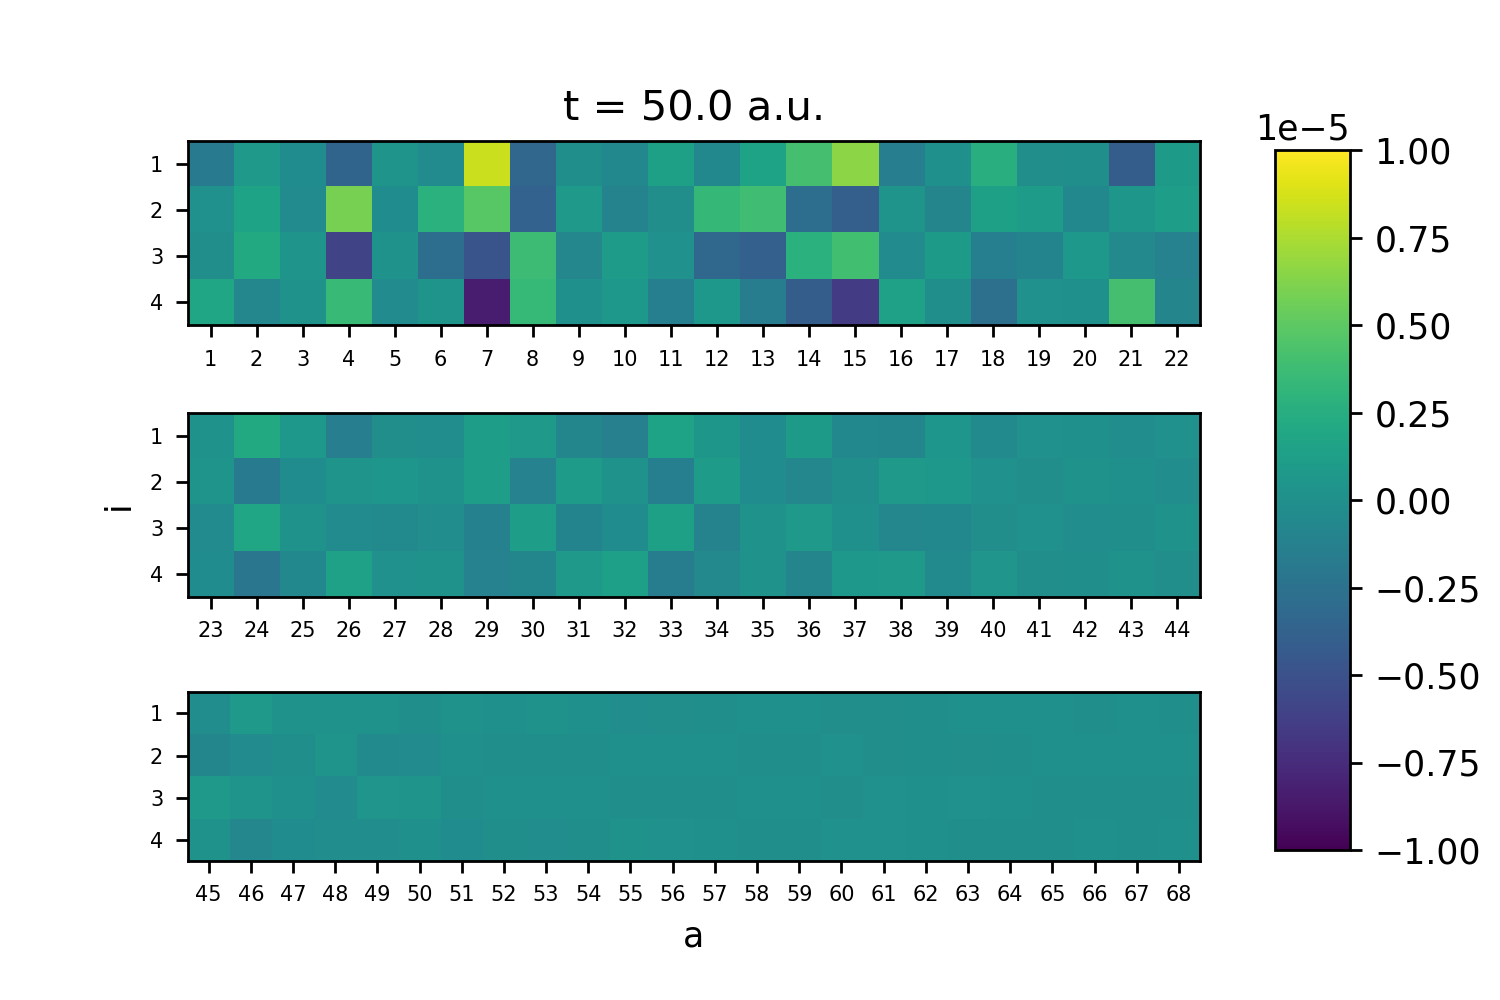
\includegraphics[scale=0.5]{p3/figures/MO_delta_t1_50.png}
        \caption{}
        \label{fig:MO_t1_50}
    \end{subfigure}
    \begin{subfigure}{.5\textwidth}
        \centering
        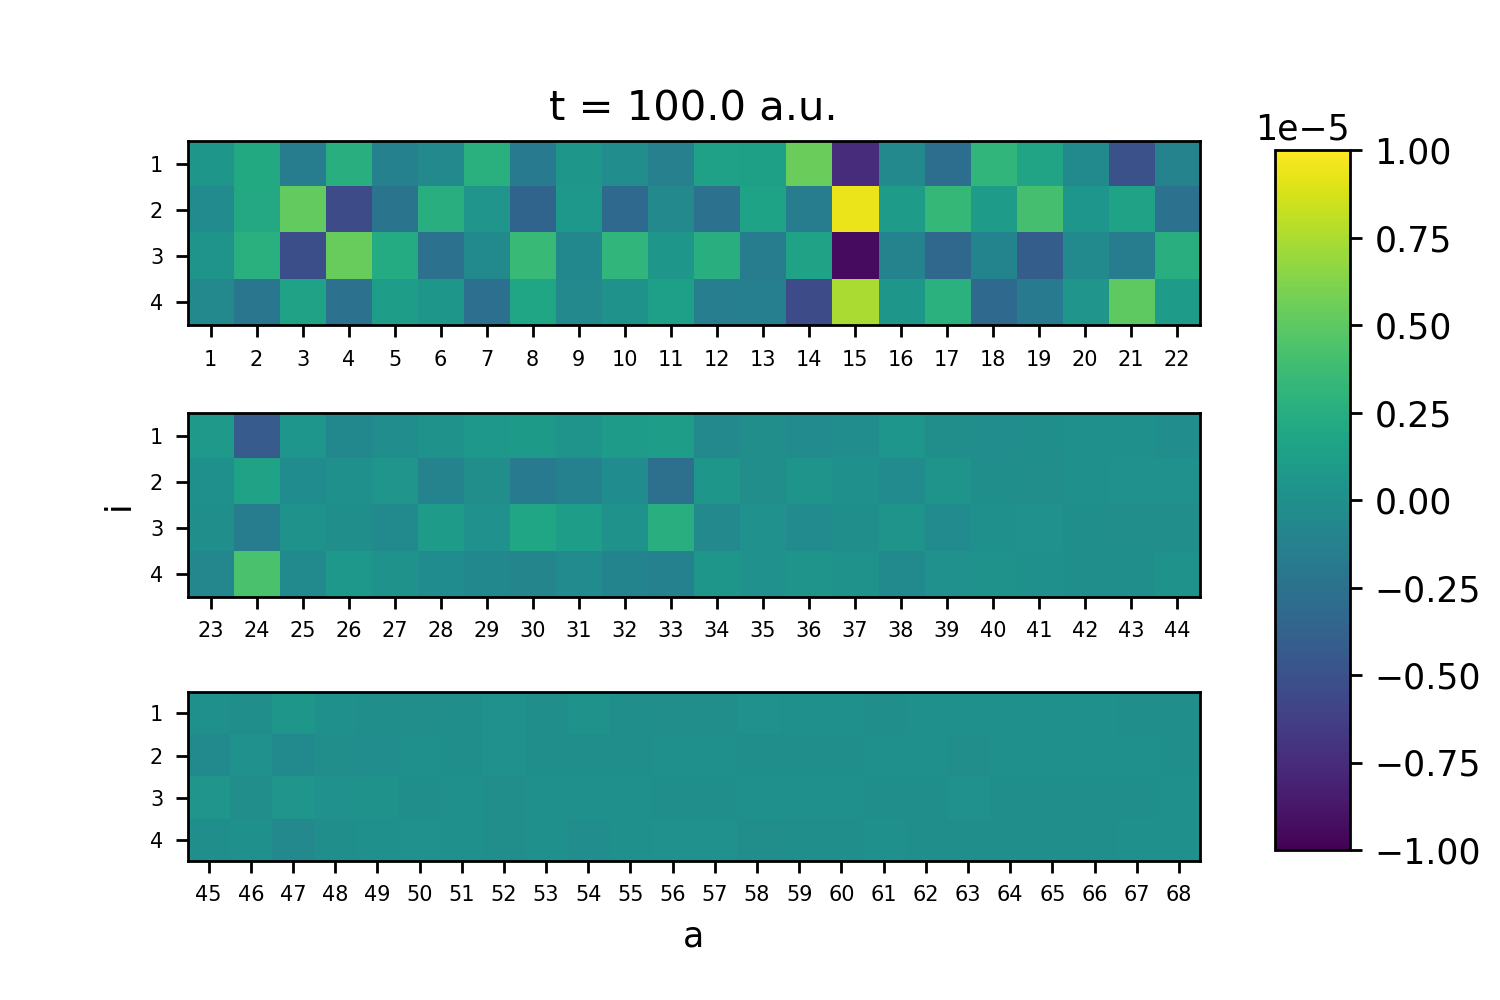
\includegraphics[scale=0.5]{p3/figures/MO_delta_t1_100.png}
        \caption{}
        \label{fig:MO_t1_100}
    \end{subfigure}
    \caption{MO-basis $t_1$ amplitude deviations from $t = 0$ after (a) 1 a.u., (b) 50 a.u., and 
    (c) 100 a.u. of time propagation. Each row contains the same four occupied orbital indices
    and a subset of virtual indices as indicated by the x-axis labels.}
    \label{fig:amps}
\end{figure}
The amplitudes are ordered by the orbital energies of the associated MOs. 
The amplitudes which experience significant oscillations vary throughout the simulation,
though there are several discernible trends. First, most large amplitude deviations
are associated with all occupied orbitals simultaneously. This is due to the relatively small size of 
the system, with only four occupied orbitals, all of which are likely important in the
description of the ground- and excited-state wave functions. Secondly, 
at any given time during the propagation,
a large number of amplitudes have not significantly deviated from their ground state values.
This supports the notion
that relative sparsity is maintained within the amplitudes throughout the simulation,
but this sparsity is distributed differently throughout the amplitude tensors as
the wave function is propagated.  

A third trend is that amplitudes which respond strongly tend to be associated with 
low-energy virtual orbitals. Chemical intuition would suggest that energetically 
low-lying molecular orbitals will be the most involved in electronic excitations.
However, while amplitude responses are indeed larger for lower-energy virtual orbitals, 
smaller amplitude 
deviations in Figure~\ref{fig:amps} extend far into the virtual space. This explains
the difficulty of simply truncating with respect to orbital energy: the 
high-energy MOs are still important to the time-evolution of the wave function 
in the presence of an EMF. 

Figure~\ref{fig:pno_amps} shows the $t_1$ amplitudes for the same simulation,
rotated into the untruncated PNO basis using $Q_{ii}$ as defined in
Eq.~(\ref{eq:Q_pno}).
\begin{figure}
    \begin{subfigure}{.5\textwidth}
        \centering
        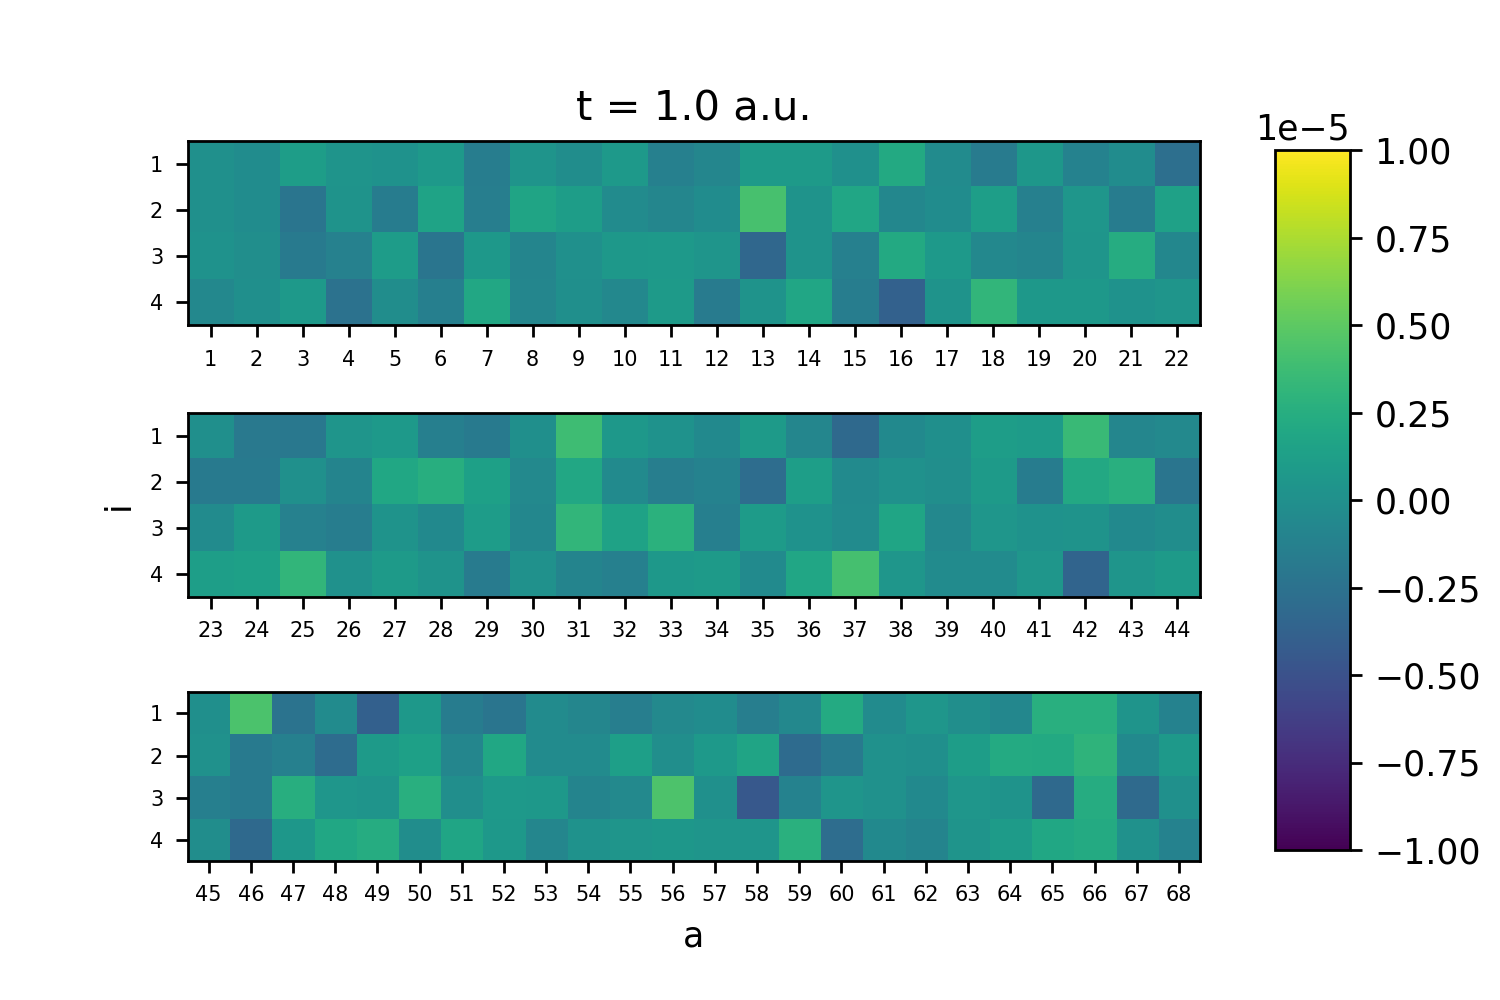
\includegraphics[scale=0.5]{p3/figures/PNO_delta_t1_1.png}
        \caption{}
        \label{fig:PNO_t1_1}
    \end{subfigure}%
    \begin{subfigure}{.5\textwidth}
        \centering
        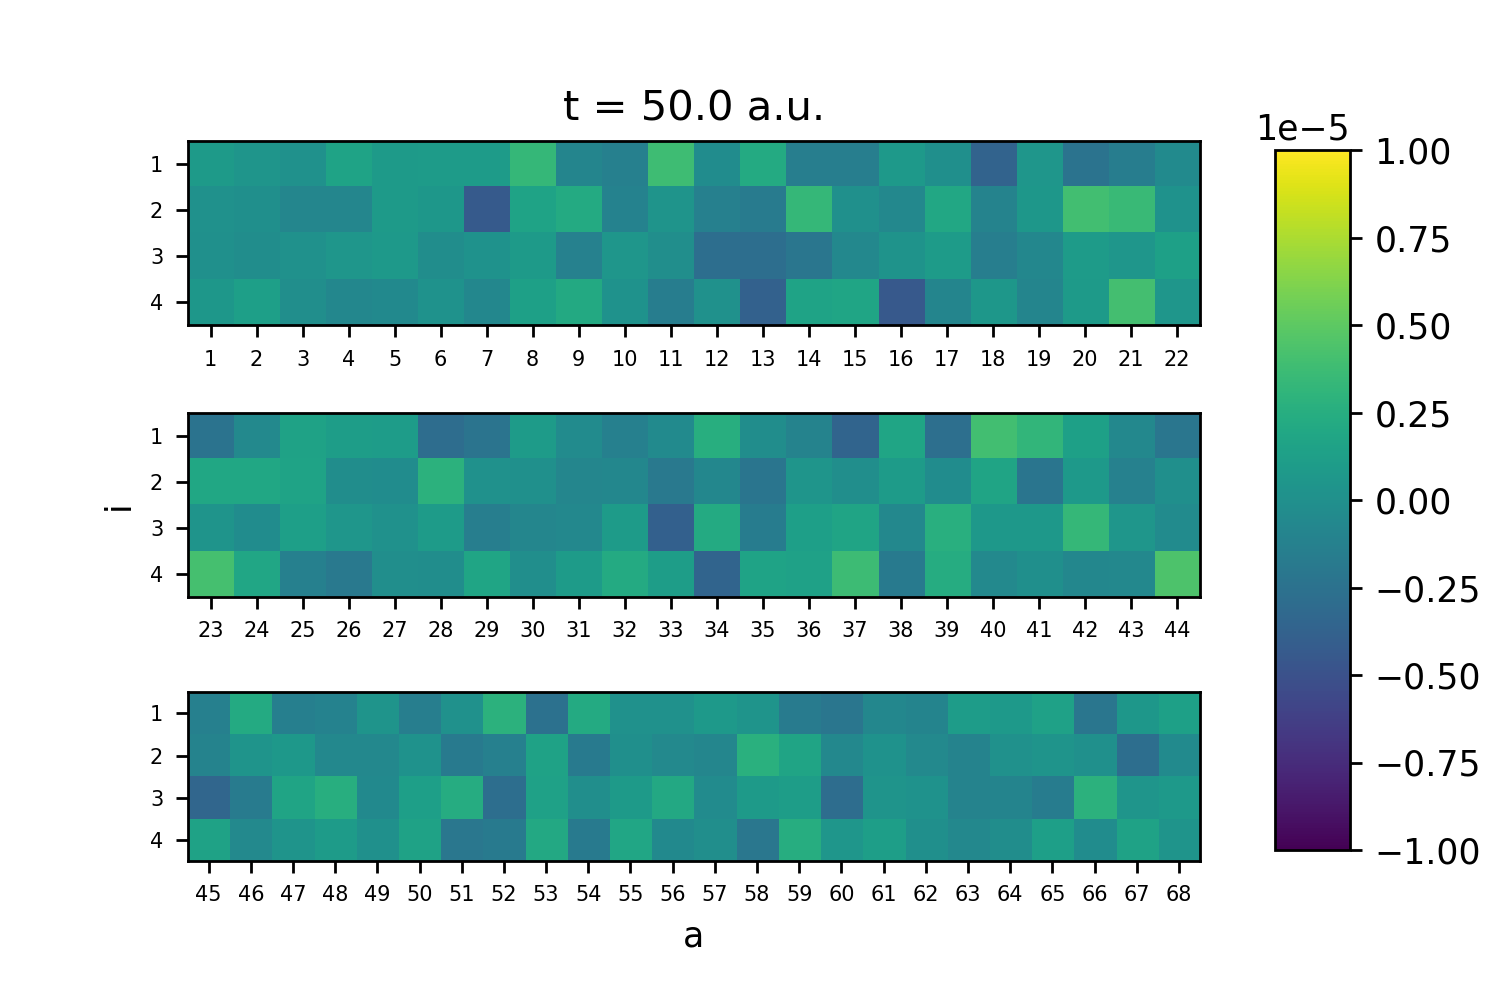
\includegraphics[scale=0.5]{p3/figures/PNO_delta_t1_50.png}
        \caption{}
        \label{fig:PNO_t1_50}
    \end{subfigure}
    \begin{subfigure}{.5\textwidth}
        \centering
        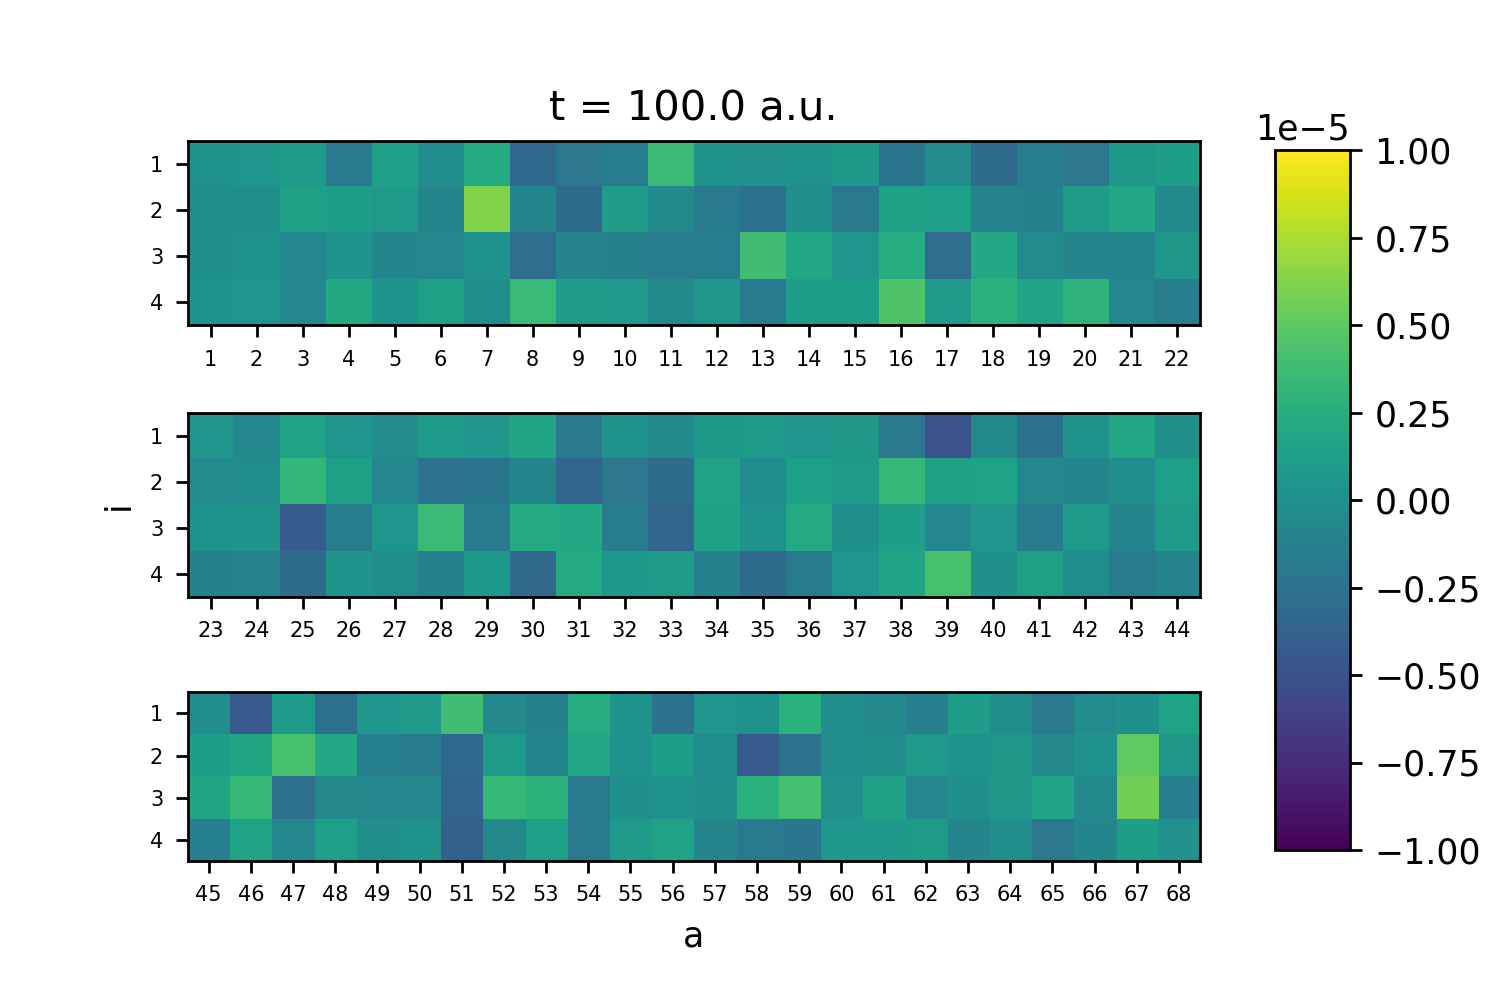
\includegraphics[scale=0.5]{p3/figures/PNO_delta_t1_100.png}
        \caption{}
        \label{fig:PNO_t1_100}
    \end{subfigure}
    \caption{PNO-basis $t_1$ amplitude deviations from $t = 0$ after (a) 1 a.u., (b) 50 a.u., and 
    (c) 100 a.u. of time propagation. Each row contains the same four occupied orbital indices
    and a subset of virtual indices as indicated by the x-axis labels.}
    \label{fig:pno_amps}
\end{figure}
(It should be noted that, due to redundancy in the AO-based virtual 
spaces for each pair, PAO-basis amplitudes cannot be compared directly in 
this manner.)
It can be immediately seen that the amplitude deviations
are less sparse in the PNO basis after the application of the EMF. 
Many more amplitudes exhibit
perceivable differences, and strong deviations (magnitudes approaching 
$1\times 10^{-5}$) are no longer present. This is a clear demonstration
of the issue with truncating orbital spaces based on the present criterion ---
rather than exploiting sparsity, the amplitude tensors have become less sparse.
%It may also suggest a recipe for building a more appropriate 
%virtual space for truncation. 
%In the following section, we propose some alternative schemes based on the 
%literature and the results of this study.

%\subsection{Possible Alternatives} \label{ss:alt}
\begin{figure}
    \centering
    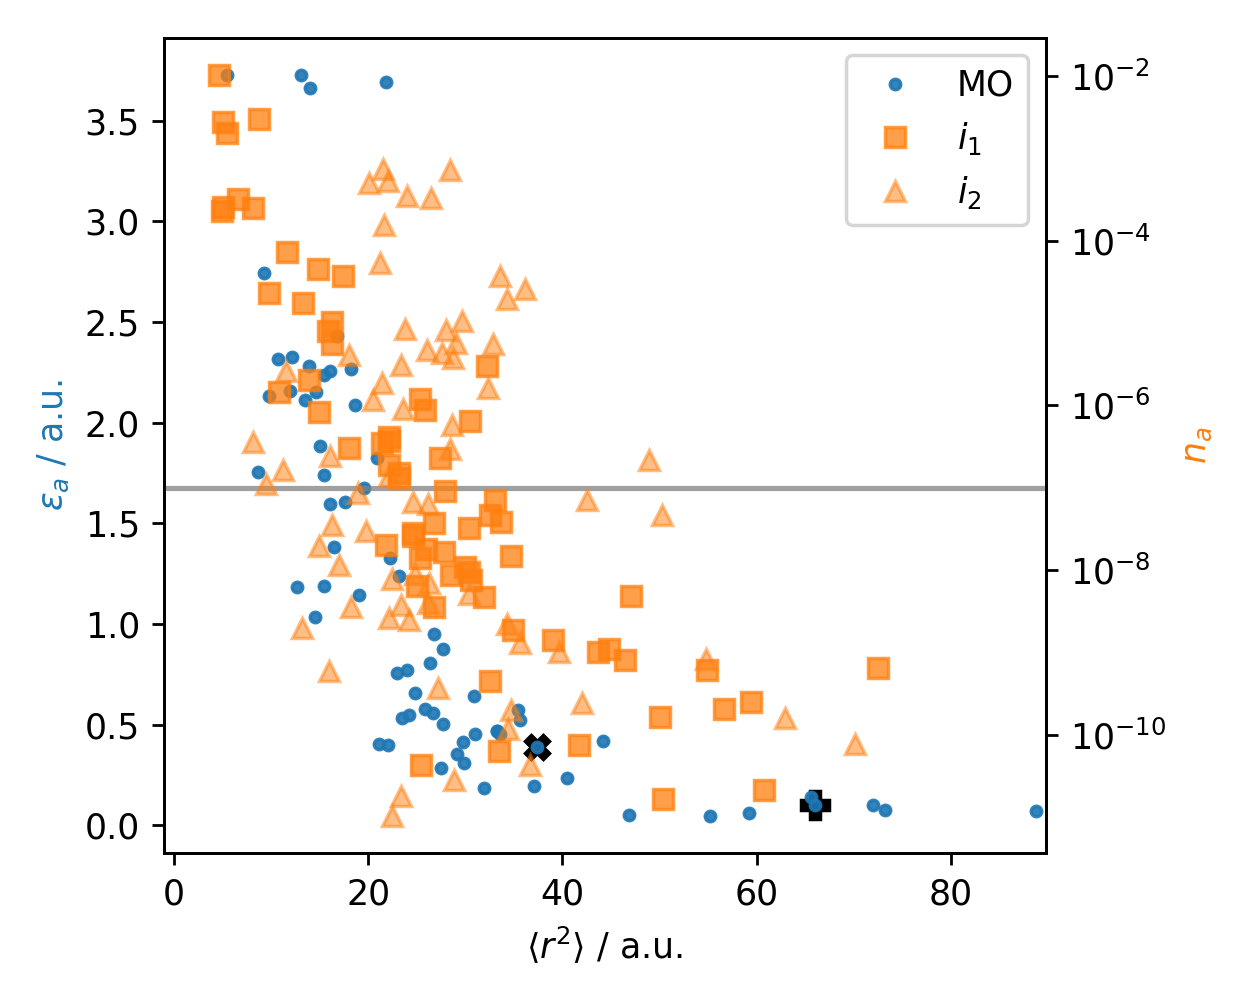
\includegraphics[scale=0.75]{p3/figures/extent.png}
    \caption{Virtual MO energy $\epsilon_a$ and the
    occupation number $n_a$ (plotted on a log scale)
    for unique PNO spaces $i_1$ and $i_2$ 
    versus orbital extent.
    Virtual MOs 7 and 15 are denoted by a solid $\boldsymbol{+}$ 
    and $\boldsymbol{\times}$, respectively.
    The horizontal line denotes a PNO cutoff 
    of $1\times 10^{-7}$.}
    \label{fig:extent}
\end{figure}
Virtual orbital extent has been used previously\cite{Kumar2017,DCunha2021} 
to estimate the ability of locally correlated spaces to describe the 
diffuse regions of electron density which are important for response
properties. 
Figure~\ref{fig:extent} shows the virtual MO energy $\epsilon_a$ and the 
PNO occupation number $n_a$ plotted against the orbital extent
$\langle r^2 \rangle$ in a.u. 
In the PNO basis, a unique virtual space is prepared
for every occupied pair, resulting in 16 unique spaces for the four occupied
spatial orbitals $i$. However, for transforming
a single orbital index, we only require the diagonal rotation matrices,
\textit{i.e.}, $Q_{ii}$. There are four such spaces; however, by symmetry,
only two are unique. Both are included in Figure~\ref{fig:extent}. 

Truncation of the PNO space begins from the bottom of Figure~\ref{fig:extent}. 
At an occupation number cutoff of $1\times 10^{-7}$ (indicated by a horizontal
line), all orbitals below this line are neglected in the PNO space. Roughly
66\% of the virtual space lies in this region. From these data, it is clear
that even modest truncation of the virtual space neglects the diffuse 
regions of the wave function, which are important for excited-state
properties in systems with significantly delocalized characteristics,
such as systems containing Rydberg-type excitations.

Spatial extent alone may not be a suitable criterion for truncation --- 
this would have a negative impact on the accuracy of the 
correlation energy, which is inherently local in nature. 
Additionally, contracted orbitals may very well contribute 
significantly to the response of the wave function. 
Figure~\ref{fig:extent} highlights virtual MOs 7 
($\boldsymbol{+}$) and 15 ($\boldsymbol{\times}$).
These orbitals correspond to the strongest deviations in 
Figures~\ref{fig:MO_t1_50} and \ref{fig:MO_t1_100}, respectively.
These deviations represent a strong response of the wave function
to the perturbing field, implying they are of particular importance
when computing dynamic properties. 
Examination of the spatial extents of these orbitals in particular 
may shed light on the nature of the spatial distribution of 
orbitals necessary to describe the wave function response.
Virtual MO 7 appears at 66 a.u., while MO 15 is nearly half that at 37 a.u.
That these orbitals are of such varying extent
demonstrates that both diffuse and contracted orbitals play a role in 
the wave function dynamics.

